\lecture{10}{Диаграмма Вороного.}
\subsection{Диграмма Вороного.}
Пусть на плоскости задано множество $S$, содержащее $N$ точек $p_1, p_2, \ldots, p_{n}$.
\begin{definition}
  \highlight{Диаграмма Вороного} --- разбиение $\R^2$ на геометрические места точек $V_1, V_2, \ldots, V_{n}$,
  в каждом из которых $p_{i}$ --- ближайшая точка.
\end{definition}
\begin{figure}[H]    
  \centering    
  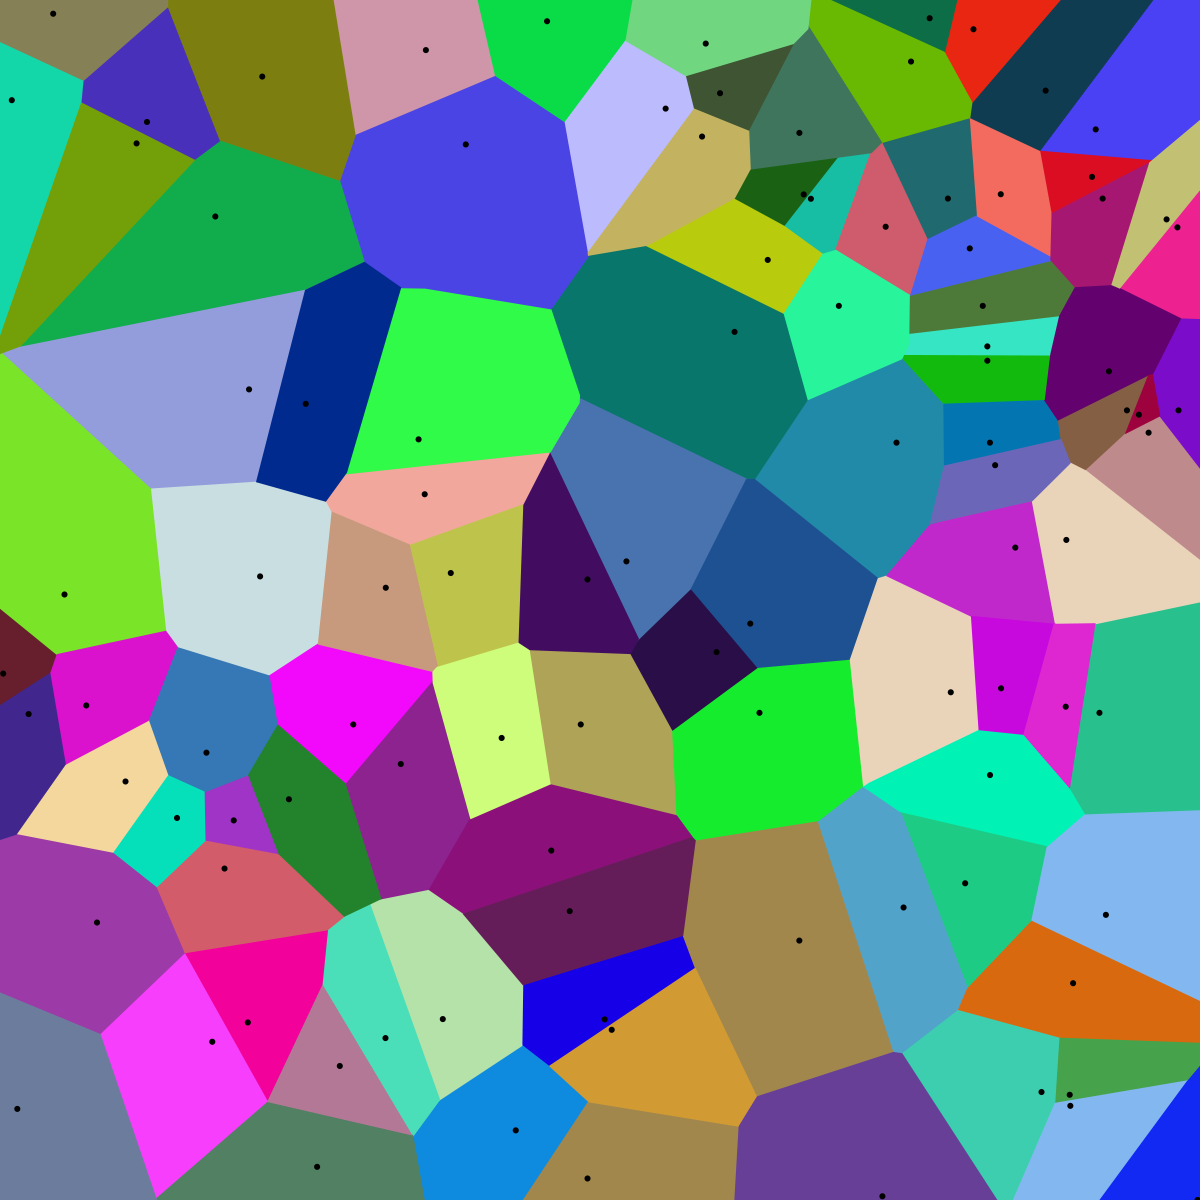
\includegraphics[width=0.5\textwidth]{figures/voronoiExample.png}    
  \caption*{Пример диаграммы Вороного}        
\end{figure} 

\begin{definition}
  \highlight{Многоугольник Вороного} --- многоугольник, образованный пересечением полуплоскостей точек,
  более близких к $p_{i}$, нежели чем к $p_{j} \in A$, где $A$ --- множество всех точек. Или же
  клеточка диаграммы Вороного.
\end{definition}

\subsection{Связь с триангуляцией Делоне.}
\begin{theorem}
  Ребро $x_{i}x_{j}$ принадлежит некоторому треугольнику триангуляции Делоне $\iff$ некоторый отрезок
  серединного перпендикуляра к $x_{i}x_{j}$ является ребром диаграммы Вороного.
\end{theorem}
\begin{figure}[H]    
  \centering    
  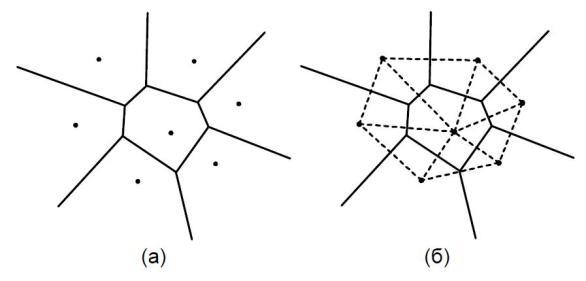
\includegraphics[width=0.5\textwidth]{figures/voronoiDelone.jpg}    
  \caption*{Связь диаграммы Вороного и триангуляции Делоне}        
\end{figure} 

\subsection{Построение диаграммы Вороного через оболочку.}
\begin{enumerate}
  \item Проектируем точки на параболоид
  \item Строим 3D выпуклую оболочку, получаем триангуляцию Делоне
  \item Из триангуляции получаем диаграмму Вороного
\end{enumerate}

\subsection{Алгоритм Форчуна.}

Данный алгоритм поддерживает заметающую прямую (по аналогии со ScanLine), а также береговую линию, которая
состоит из различных парабол и кусков парабол. Пусть все точки слева от заметающей прямой обработаны, 
тогда береговая линия отделяеn порцию плоскости, внутри которой диаграмма Вороного может быть известна,
независимо от других точек справа.

\begin{figure}[H]    
  \centering    
  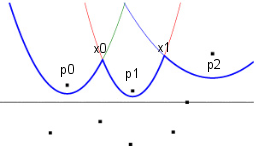
\includegraphics[width=0.5\textwidth]{figures/forchExample.png}    
  \caption*{Пример для понимания береговой линии (только здесь она горизонтальная)}        
\end{figure} 

Для каждой точки слева от заметающей прямой можно определить параболу, которая равноудалена как от этой
точки, так и от заметающей прямой. Тогда заметающая прямая будет директрисой для параболы, а точка --- 
фокус. По мере движения прямой, вершины береговой линии в которых две параболы пересекаются, вычерчивают
рёбра диграммы Вороного. 

При движении прямой мы заносим в очередь с приоритетом события, которые могли бы изменить структуру
береговой линии (например, добавление новой параболы, т.е. появление новой точки, а также пересечение
серединных перпендикуляров --- исчезновение одной параболы), а также храним структуру береговой линни
в дереве. Алгоритм состоит из последовательного удаления события из очереди с приоритетом, нахождения
изменений событий в береговой линии и обновления структуры данных.

\begin{remark}
  Асимптотика алгоритма $O(n \log n)$. Всего у нас $O(n)$ событий для обработки (каждое будет ассоциировано
  с некоторым свойством диаграммы Вороного) и на каждое событие $O(\log n)$ времени для обработки.
\end{remark}

